
\chapter{Motivations}

The existence of additional $U(1)$ gauge symmetries of nature are common in
several Beyond the Standard Model (BSM) theories 
\cite{Goodsell:2010ie, Abel:2008ai, Candelas:1985en, Andreas:2011in, Jaeckel:2010ni}.
Such theories envision the associated gauge boson  inhabiting a  ``hidden sector'' 
consisting of a complex of 
particles and gauge bosons.  Probing the structure of such a hidden sector may
be possible through the so called ``Vector'' portal which describes  
the weak coupling of the $A'$ to charged particles through ``kinetic mixing''
with the photon. In fact, it is natural for the $A'$ to 
kinetically mix with the Standard Model (SM) photon through the interaction
of massive fields carrying both SM hypercharge and dark charge \cite{Holdom:1985ag}.
The mixing of the photon with the $A'$ would not only allow searching for
new hidden sector particles, but also for dark matter which some theoretical models
have envisioned as inhabiting the hidden sector, with its interactions mediated
via an $A'$ 
\cite{ArkaniHamed:2008qn, Pospelov:2008jd, cheung2009, ArkaniHamed:2008qp}.

The chapter that follows will motivate the need to search for an $A'$.  
This includes an overview of current astrophysical anomalies
that may be explained assuming a dark matter candidate that couples to a 
heavy photon.  Finally, a review of current experimental limits on the $A'$ 
coupling strength will be given.

\section{Theoretical Formalism and Physics Motivation}

As Holdom \cite{Holdom:1985ag} formulated in the mid eighties, in a theory with 
$U(1)_Y \times U(1)'$ symmetry, there is a term in the gauge part of the Lagrangian 
that allows $U(1)_Y$ and $U(1)'$ to mix.  The gauge part of such a theory can
be written as
\begin{equation}
    \mathcal{L}_{\text{gauge}} = - \frac{1}{4} F_Y^{\mu \nu}F_{Y, \mu \nu}
                          - \frac{1}{4} F'^{\mu \nu}F'_{\mu \nu}
                          + \frac{1}{2} \epsilon F'^{\mu \nu} F_{Y, \mu \nu}
    \label{eqn:l_gauge}
\end{equation}
where $F'_{\mu \nu} = \partial_{\mu}A'_{\nu} - \partial_{\nu}A'_{\mu}$ 
($F^{\mu \nu}_{Y} = \partial^{\mu}A^{\nu} - \partial^{\nu}A^{\mu}$) is the
field strength tensor of the heavy photon (SM hypercharge) and $\epsilon$ is a
dimensionless coupling constant.  Illuminating the low-energy effects that result
from kinetic mixing can be achieved by decoupling the gauge fields through the
redefinition of the SM hypercharge gauge field as
\begin{equation}
    A_{\mu} \rightarrow A_{\mu} + \epsilon A'_{\mu}.
\end{equation}
Ignoring all $\epsilon^2$ terms that arise from such a transformation, this
results in the diagonalization of Equation \ref{eqn:l_gauge} as
\begin{equation}
    \mathcal{L}_{\text{gauge}} = - \frac{1}{4} F_Y^{\mu \nu}F_{Y, \mu \nu}
                          - \frac{1}{4} F'^{\mu \nu}F'_{\mu \nu}.
\end{equation}
However, the redefinition of the field also affects the interaction term of 
the Lagrangian, $\mathcal{L}_{int} = A^{\mu}J_{\mu}^{EM}$ as
\begin{equation}
    A^{\mu}J_{\mu}^{EM} \rightarrow (A^{\mu} + \epsilon A'^{\mu})J_{\mu}^{EM}.
\end{equation}
As a result, an effective coupling is induced between the electromagnetic 
current and the heavy photon field that is suppressed by a factor of $\epsilon$.

%If $U(1)_Y$ is embedded in a Grand Unified Theory such as $SU(5)$, kinetic mixing between the
Mixing between the
SM photon and the heavy photon can naturally be generated at loop-level,
assuming there exist heavy multiplets, ($\Phi$, $\Phi'$), 
that are charged under both the SM hypercharge and dark charge 
(see Figure \ref{fig:ap_loop}).
\begin{figure}
    \centering
    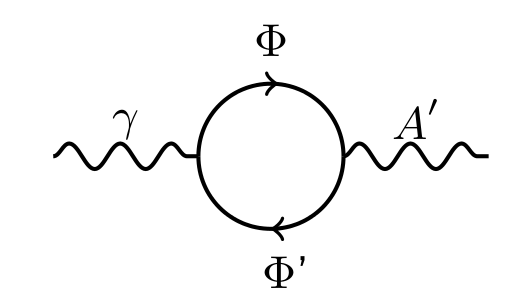
\includegraphics[width=0.5\textwidth]{images/aprime_loop.png}
    \caption{Kinetic mixing of a Standard Model photon with a heavy photon 
    at one-loop through the interaction of massive fields charged under
    the Standard Model hypercharge and dark charge.}
    \label{fig:ap_loop}
\end{figure}
Integrating out the fields generates values of $\epsilon$ on the order of 
\begin{equation}
    \epsilon \sim \frac{g_Yg_D}{16\pi^2}\ln\left(\frac{m_{\Phi}}{m_{\Phi'}} \right)
             \sim 10^{-3} - 10^{-1} 
\end{equation}
where $g_Y$ ($g_D$) are the SM hypercharge (dark) coupling and 
$(m_{\Phi}, m_{\Phi'})$ are the masses of the two fields 
\cite{ArkaniHamed:2008qp, Bjorken:2009mm}.  If the theory doesn't contain 
split multiplets charged under both $U(1)_Y$ and $U(1)'$, the mass splittings 
can be generated by additional loops, leading to values of $\epsilon \sim 10^{-6} - 10^{-3}$. 
In some string theory constructions, 
values as small as $\epsilon \sim 10^{-12}$ are expected 
\cite{Goodsell:2010ie,Goodsell:2009xc, Cicoli:2011yh}.

%
% If I have time, I need to add a paragraph explaining how an A' would acquire
% mass.
%

The possibility that a new gauge boson can couple to charged SM particles is 
very appealing.  It may offer one of the few portals to probe a new sector 
composed of light weakly coupled particles and possibly dark matter
(see Section \ref{sec:mot_dm}).  Such a coupling can be exploited by current and future
experimental programs in order to measure the properties of
the hidden sector and possibly provide insight into many outstanding physics 
puzzles.

\section{Motivations for a Heavy Photon from Dark Matter} \label{sec:mot_dm}

Although the existence of dark matter (dark matter) has been firmly established through its
gravitational interaction 
\cite{Zwicky:1933gu, Rubin:1980zd, Clowe:2006eq, Adam:2015rua}, its exact nature
continues to elude us. An appealing
possibility is that dark matter inhabits a ``hidden sector'' with its interactions 
mediated by an $A'$.  In turn, the kinetic mixing of the $A'$ with the SM 
photon may provide a portal that would allow the exploration of not only the 
properties of dark matter but the hidden sector itself.  Furthermore, several recently
observed astrophysical anomalies \cite{Adriani:2008zr, ackermann2012, aguilar2013, 
hooper2011, linden2011, abazajian2012, hooper2013, Bulbul:2014sua}
may have a dark matter interpretation if dark matter is
charged under $U(1)'$.  A summary of those anomalies along with their dark matter
interpretation will be presented here.

\subsection{Cosmic Rays}

Interest in hidden sector models surged in 2008 with the announcement by 
PAMELA of an unforeseen rise in the ratio of the cosmic ray (CR) positron flux
to CR electron flux, $e^{+}/(e^{+} + e^{-})$, above 10 GeV \cite{Adriani:2008zr}.
The rise was later confirmed by both the 
Fermi Gamma-Ray Space Telescope \cite{ackermann2012} and Alpha Magnetic 
Spectrometer-02 (AMS-02) \cite{aguilar2013} experiments and observed to continue
up to 200 GeV. 

The main source of CR positrons 
was expected to come from the interaction of CR nuclei with the interstellar 
medium (secondary production).  If such a production mechanism was dominant, 
cosmic ray propagation models predicted the fraction would fall with increasing
energy.  The observed rise immediately led to the speculation of additional sources of 
positrons \cite{yin2013, linden2013}.

One attractive scenario that could account for the rise is the annihilation of
dark matter to leptons ($e^+e^-, \mu^+\mu^-$). In fact, such models where found to fit 
the data fairly well but require much 
larger annihilation rates compared to those expected assuming the typical 
thermal cross-section \cite{Cholis:2008hb}
\begin{equation}
    \left \langle \sigma v \right \rangle \simeq 3 \times 10^{-26} \text{cm}^3 \text{s}^{-1}.
\end{equation}

Alternatively, if dark matter interactions are mediated by a heavy photon, a 
``Sommerfeld enhancement'' of the annihilation cross-section proportional to
$\langle \sigma v \rangle \sim 1/v$ can occur \cite{ArkaniHamed:2008qn}. 
In such scenarios, the
``freeze-out'' cross-section that leads to the currently observed relic
abundance remains unaffected since the velocity of dark matter in the early universe was
high and the Sommerfeld enhancement had not effectively turned on.  If the 
heavy photons created in the annihilation of dark matter subsequently decay to leptons
(Figure \ref{fig:dm_annihilation}), the resulting $e^+e^-$ spectrum could
account for the rise.  Using the latest AMS-02 results, such a model can 
accommodate the data only if the mass and annihilation 
cross-section of dark matter ranges between $\sim$ 1.5 - 3 TeV and 
$\langle \sigma v \rangle \sim (6-23) \times 10^{-24}$ cm$^{-3}$/s 
\cite{Cholis:2013psa}. 
\begin{figure}[t]
    \centering
    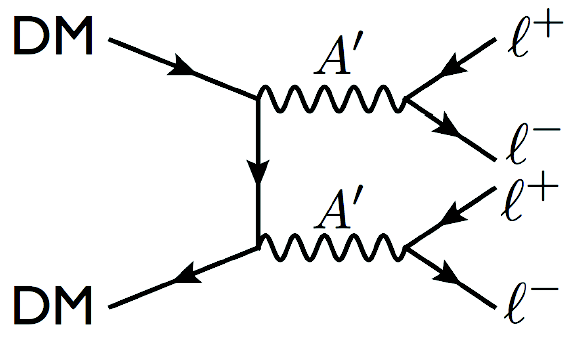
\includegraphics[width=0.5\textwidth]{images/dm_annihilation.png}
    \caption{Diagram of dark matter annihilation to a heavy photon which subsequently 
             decays into a pair of leptons.}
    \label{fig:dm_annihilation}
\end{figure}

The most recent measurement of the cosmic microwave background (CMB) by the
Planck satellite strongly disfavor dark matter annihilation as the cause of 
the CR excess \cite{Ade:2015xua}.  The annihilation of dark matter in the early
universe 
injects extra energy into the primordial plasma.  This would increase the 
fraction of hydrogen that was ionized during recombination, resulting in a 
modification of the CMB spectrum.  Thus, a constraint on the annihilation 
cross-section of dark matter can be obtained through the measurement of the
CMB anisotropy.  

\subsection{Light Dark Matter}

Recently, an analysis of three years of data collected by the Fermi Large Area
Telescope observed an extended emission in the spectrum of gamma-rays 
originating from the Galactic Center 
\cite{hooper2011, linden2011, abazajian2012, hooper2013}.  Several models have been 
devised to try to explain the emission including the collision of energetic 
protons accelerated by a super-massive black hole \cite{Hooper:2010mq}, 
pulsars \cite{Abazajian:2010zy} and dark matter annihilation to leptons or 
hadrons \cite{Hooper:2010mq, Goodenough:2009gk}.  The emission can also
be explained in the context of dark matter annihilating to an $A'$ which 
subsequently decays to SM particles \cite{Hooper:2012cw}.  Such a model assumes
a dark matter candidate of mass $\sim$ 10 GeV annihilating to a heavy photon
with a mass $\sim$ 100 MeV. 

Another anomaly that can be explained in the context of a light dark matter
candidate that couples to a heavy photon is the observation
of a 3.5 keV X-ray line in the spectrum of 73 galaxy clusters \cite{Bulbul:2014sua}.  
Specifically, the ``eXciting Dark Matter'' model \cite{Finkbeiner:2014sja} 
proposes the existence of a doublet of dark matter states whose self interactions are 
mediated by a heavy photon. As shown of Figure \ref{fig:dm_self_scat}, a pair
of dark matter particles upscatter via an $A'$ to produce a pair of excited states, 
$\chi^*\chi^*$. This is immediately followed by the decay 
$\chi^* \rightarrow  \chi\gamma$, producing an X-ray line.
\begin{figure}[t]
    \centering
    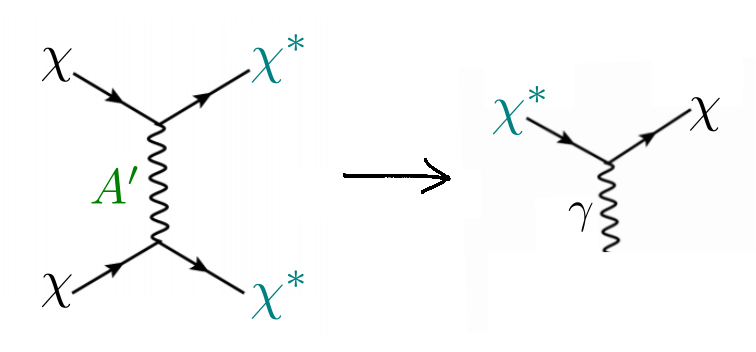
\includegraphics[width=0.9\textwidth]{images/xdm.png}
    \caption{A diagram depicting the self-scattering of dark matter via a heavy
             photon into an excited state. The excited state subsequently decays
             producing an observable X-ray line.}
    \label{fig:dm_self_scat}
\end{figure}


\section{Current Limits on Heavy Photons} \label{sec:current_limits}

As previously discussed, a heavy photon with a mass between 1 MeV and 1 GeV and
$\epsilon$ as small as $10^{-12}$ is well motivated by both theoretical
considerations and recent astrophysical anamolies.  A major portion of this
region in the mass-coupling phase-space remains hitherto unexplored. However,
several experiments will be taking place in the coming years with the intention
to probe this favorable portion of phase space. These include HPS, APEX \cite{Essig:2010xa}, 
DarkLight \cite{Freytsis:2009bh}, VEPP-3 \cite{Wojtsekhowski:2012zq},
MESA \cite{Beranek:2013yqa}, Mu3e \cite{Echenard:2014lma}, 
SeaQuest \cite{Gardner:2015wea}, SHiP \cite{Alekhin:2015byh}, Belle-II and 
LHCb \cite{Ilten:2016tkc, Ilten:2015hya}.

Existing $2\sigma$ significance constraints
from beam dump \cite{Bjorken:1988as, riordan1987, bross1991, konaka1986,
                     davier1989, Bjorken:2009mm, andreas2012, Blumlein:1990ay,
                     Blumlein:1991xh, johannes2011, johannes2014},  
collider \cite{Reece:2009un, Aubert:2009cp, Babusci:2012cr, Archilli:2011zc} 
and fixed target experiments \cite{Abrahamyan:2011gv, Merkel:2014avp,
                                   Agakishiev:2013fwl, Batley:2015lha}
on heavy photons with a mass and coupling in the favorable region are shown 
in Figure \ref{fig:ap_limits}. The regions labeled ``$a_e$'' and ``$a_\mu$'' 
are exclusions based on the muon and electron $g-2$.
The green band labeled ``$a_{\mu} \pm 2\sigma$ favored'' represents the region
that an $A'$ can be used to explain the discrepancy  between the measured and
calculated muon anomalous magnetic moment \cite{Pospelov:2008zw, Bennett:2006fi}.
The experimental searches for heavy photons will be discussed in more detail
in the sections that follow.

\subsection{Electron Beam Dump Experiments}

Electron beam dump experiments make use of a high intensity beam ``dumped'' onto
a thick ($\sim$cm) target to produce highly boosted heavy photons through a 
process analogous to photon bremsstrahlung.  In order to suppress the large
SM backgrounds produced at the target, a shield of thickness between 1 and 
100 cm
%$\sim$cm - m
is placed immediately downstream of the target, and in front of the detector.  Since the 
heavy photons interact weakly with SM particles, sufficiently long lived 
heavy photons will traverse the shield before reaching an open space upstream
of a detector.  The decay products of heavy photons decaying in this region 
will travel unimpeded until detected.
The thickness of the target and shield in combination with a high luminosity
beam allow such experiments to be sensitive to heavy photons with small 
couplings which tend to travel considerable distances before decaying. Such 
experiments tend to be sensitive to heavy photons which have a mass on the order
of 100 MeV and a coupling in the range $10^{-7} \le \epsilon \le 10^{-3}$.  
Sensitivity to larger couplings is limited by the lifetime of the $A'$ since
short lived heavy photons will decay in the shield.

% What backgrounds are these experiments concerned with?
% What is the shield made of?

Several electron beam dump experiments were devised over the last several decades with
the intention of searching for axions \cite{Peccei:1977hh} \footnote{Axions are particles postulated 
by Peccei and Quinn in the late 70's in an attempt to resolve the strong CP problem.}.  These 
included E137 \cite{Bjorken:1988as}
and E141 \cite{riordan1987} conducted at SLAC National Accelerator Laboratory,
E774 \cite{bross1991} at Fermi National Accelerator Laboratory, and experiments at 
KEK \cite{konaka1986} in Japan and Orsay \cite{davier1989} in France. 
%The setup of each of the experiments is summarized on Table \ref{}. 
The results from each of these experiments have been reinterpreted in the 
context of a search for a heavy photon and used to set limits on the coupling
strength $\epsilon$ \cite{Bjorken:2009mm, andreas2012}.  
%The resulting limits are 
%shown in Figure \ref{fig:ap_limits}.

\subsection{Proton Beam Dump Experiments}

Proton beam dump experiments can also be used to search for heavy photons
through either the decay of neutral mesons produced at the target or proton
bremsstrahlung. One such experiment, performed at the U70 accelerator at IHEP
Serpukhov, used a 68.6 GeV proton beam incident on an iron target 
%The data collected by one such experiment that used the U70
%accelerator at IHEP Serpukhov, was originally devised 
to search for axions
and a light Higgs boson \cite{Blumlein:1990ay, Blumlein:1991xh}.  The data
collected by the experiment were reanalyzed, and used to search for a heavy photon.
Specifically,
The myriad of $\pi_0$ mesons produced at the target were used to search for an 
$A'$ using the $\pi_0 \rightarrow A'\gamma (A' \rightarrow e^+e^-)$ 
decay channel \cite{Blumlein:2011mv}.  Furthermore, the production of heavy
photons through proton bremsstrahlung was also used to search for an 
$A' \rightarrow e^+e^-$ \cite{Blumlein:2013cua}.

\subsection{Colliders}

The past few decades saw the operation of several high-luminosity $e^+e^-$ colliders 
that were able to collect data at different center-of-mass energies.
These include KLOE, running at the the DA$\Phi$NE $\phi$ factory, and BaBar 
at the PEP-II B-Factory. Searches at BaBar were performed using the channel 
$e^+e^- \rightarrow A' \gamma (A' \rightarrow \mu^+\mu^-)$ 
\cite{Reece:2009un, Aubert:2009cp}.  KLOE 
searched for heavy photons in the decays of the $\phi$ meson.  Specifically, 
the channel $\phi \rightarrow \eta A' (A' \rightarrow e^+e^-)$ was used to
set limits on the coupling strength of the $A'$ 
\cite{Babusci:2012cr, Archilli:2011zc}.
%The limits set by both BaBar and KLOE are shown in Figure \ref{fig:ap_limits}.

The PHENIX experiment at the Relativistic Heavy Ion Collider also searched for
heavy photons using neutral meson produced in $p+p$  and $d+$Au collisions 
\cite{Adare:2014mgk}.
Specifically, the decay channels $\pi_0 \rightarrow \gamma A' (A' \rightarrow e^+e^-)$
and $\eta \rightarrow \gamma A' (A' \rightarrow e^+e^-)$ were used to set limits on the 
coupling strenght of the $A'$.

\subsection{Fixed Target Experiments}

The $A'$ production mechanism used by electron fixed target experiments is 
the same as that used by electron beam dump experiments. However, unlike beam
dump experiments, the targets used by fixed target experiments are thin allowing
such experiments to be sensitive to promptly decaying heavy photons, i.e. 
$A'$ with coupling on the order of $\epsilon \sim 10^{-3} - 10^{-1}$.
Experiments such as HPS also have the 
ability to search  for heavy photons which decay within a few cm of the target.
Thus far, fixed target searches for a heavy photon using an electron beam
have been completed by APEX \cite{Abrahamyan:2011gv} and A1 at the 
MAINZ microtron \cite{Merkel:2014avp}.

Experiments such as HADES \cite{Agakishiev:2013fwl} and NA48/2 \cite{Batley:2015lha}
can also search for heavy photons using 
neutral mesons.  Specifically, HADES used a 3.5 GeV proton beam incident on 
both a hydrogen and niobium target to produce heavy photons through the 
channels $\pi_0 \rightarrow \gamma A'$, $\eta \rightarrow \gamma A'$ and 
$\Delta \rightarrow N A'$ with the $A'$ assumed to decay to an $e^+e^-$ pair.
NA48/2 used protons extracted from CERN SPS incident on a berrylium target to 
produce a Kaon beam.  The channel $K^{\pm} \rightarrow \pi^{\pm}\pi^0 (\pi^0 \rightarrow \gamma A')$
was used to search for heavy photons.  
